%!TEX root = ../main.tex

\chapter{The physics of double-beta decay}\label{chap:theory}

Studying the properties and interactions of neutrinos has been one of the most exciting
and vigorous activities in particle physics and astrophysics ever since W.~E.~Pauli in
\yr{1930}~\cite{Brown1978}. Despite their weakly interacting nature, that challenged physicists
to detect it directly until \yr{1965}~\cite{Cowan1956}, we have so far accumulated an enormous
amount of knowledge about them. No experiments that have been performed so far have
detected conclusive deviations from the Standard Model of Particle Physics, except
neutrino oscillation experiments, which have shown that neutrinos are massive and
mixed~\cite{Fukuda1998, Ahmad2002, Eguchi2003, Kajita2016, McDonald2016}.  This discovery,
however, is far from being the last word on the fundamental properties of neutrino. The
mechanism through which the neutrino acquires mass and why it is so tiny with respect to
all the other elementary particles remains a mystery. How can such a rare nuclear process
like double-beta decay help shading some light on these enigmas?
\newpar
The mass-generation mechanism is strongly connected to the nature of these extremely light
particles, which could be either of Dirac or Majorana type (i.e.~neutrino and
anti-neutrino are distinct particles or the same particle). An attempt to address this
problem is pursued by experiments looking for the neutrinoless mode of double-beta decay.
The double-beta decay, in its two-neutrino Standard Model mode (\nnbb), consists in a
nucleus that decays into a daughter nucleus with two electrons and two electron
anti-neutrinos as a byproduct. If the neutrino is a Majorana particle then another mode
may occur (\onbb), in which neutrinos are not produced at all~\cite{Schechter1982}.
Neutrinoless double-beta decay experiments are considered the most promising way to solve
the neutrino mass puzzle, although these events are very rare processes controlled by weak
interactions.
\newpar
From its definition it is also clear that neutrinoless double-beta decay violates lepton
number conservation, an accidental symmetry of the Standard Model, by two units. The
existence of such a process beyond the Standard Model would be crucial to support
baryogenesis ideas, that aim to explain why we live in matter-dominated Universe.  Many
theories, in fact, predict that the asymmetry is eventually produced by a violation of
lepton number via leptogenesis. Neutrino Majorana masses and lepton-number violation can
be therefore verified at the same time by observing neutrinoless double-beta decay.
\newpar
Neutrinoless double-beta decay is not the only hypothetical process that can be searched
in a dedicated physics experiment. Other exotic processes have been conjectured by
theorists that have different theoretical signatures and are usually searched by studying
the distribution of two-neutrino double-beta decay events. Two of them have been
considered in this work, namely the neutrinoless double-beta decay with Majoron emission
and the Lorentz-violating two-neutrino double beta decay. The first is essentially a
variant of neutrinoless double beta decay in which massless Goldstone bosons connected to
the symmetry breaking are emitted together with the two electrons. The second one,
instead, re-considers the two-neutrino mode in the theoretical framework of an extension
of the Standard Model in which the Lorentz symmetry is not conserved.
\newpar
In the following the theory of double-beta decay is briefly reviewed, focusing on the core
concepts and formulas which will be used in this work. First, the decay scheme of the
standard two-neutrino double-beta decay mode is discussed in \cref{sec:nbb:2nbb}. The
ingredients to calculate its differential decay rate are presented, including a brief
discussion of the long-standing nuclear matrix element issue. The theoretical implications
of the hypothesized neutrinoless double-beta decay mode on the nature of the neutrino mass
and the baryogenesis puzzle are discussed in \cref{sec:nbb:0nbb}. In
\cref{sec:nbb:0nbbx,sec:nbb:2nbbLV} other exotic double-beta decay modes that contemplate
the emission of additional particles (i.e.~the Majorons) or break the Lorentz symmetry
are considered. Finally, aspects concerning the detection of double-beta decay events in
real experimental settings will be examined in \cref{sec:nbb:exp}.

\section{Standard two-neutrino double-beta decay}%
\label{sec:nbb:2nbb}

The two-neutrino double-beta decay (\nnbb) processes, first suggested by M.~Goeppert-Mayer
in \yr{1935}~\cite{GoeppertMayer1935}, can be schematically represented as:
\[
  \begin{array}{llr}
    2\upnu\upbeta^-\upbeta^-: &
      \mathcal{N}(A,Z) \longrightarrow \mathcal{N}(A,Z+2)+2e^-+2{\overline \upnu}_e & \\
    2\upnu\upbeta^+\upbeta^+: &
      \mathcal{N}(A,Z) \longrightarrow \mathcal{N}(A,Z-2)+2e^++2\upnu_e &,
  \end{array}
\]
where \NAZ\ represents a nucleus with mass number $A$ and atomic number $Z$. The \nnbbm\
(\nnbbp) process consists of the simultaneous $\upbeta^-$ ($\upbeta^+$) decay of two
neutrons (protons) in the same nucleus. The processes are generated at second-order in the
perturbative expansion of weak interactions in the Standard Model. The Feynman graph for
\nnbbm\ is shown in \cref{fig:nbb:feydiag}, left.

\begin{figure}
  \centering%
  \makebox[\textwidth]{%
    \includegraphics[width=0.5\textwidth]{plots/theory/2nbbfey.pdf}%
    \includegraphics[width=0.5\textwidth]{plots/theory/0nbbfey.pdf}%
  }
  \caption{%
    Feynman graphs for two-neutrino (left) and neutrinoless (right) double-beta decay. In
    the neutrinoless mode, the two interaction vertices are connected by a Majorana
    propagator, such that no neutrinos are present in the final state.
  }\label{fig:nbb:feydiag}
\end{figure}

Since the \nnbb\ decays have a four-body leptonic final state, the sum of the kinetic
energies of the two decay electrons follows a continuous distribution from zero to the
Q-value of the decay process (the recoil energy of the final nucleus is negligible), which
is given by
\[
  Q_{\upbeta\upbeta} = M_i - M_f - 2m_e \;,
\]
where $M_i$ and $M_f$ are, respectively, the masses of the initial and final nuclei
(i.e.~the energy levels of their ground states; if the transition occurs into an excited
energy level of the final nucleus, $M_f$ must be replaced with the appropriate energy).

A nucleus \NAZ\ can decay through a \nnbb\ process if its ground state has an energy which
is larger than the ground-state energy of the nucleus $\mathcal{N}(A,Z\pm2)$ plus twice
the electron mass. Moreover, if a nucleus can decay through both the \b\ and \nnbb\
processes, in practice the latter is not observable, because its \b\ decay lifetime is
much shorter than its \nnbb\ decay lifetime (the half-life of \nnbb\ is typically around
$10^{19}-10^{24}$ yr). Therefore, in practice the \nnbb\ decay of a nucleus is observable
only if its \b\ decay is energetically forbidden or strongly suppressed because of a large
change of spin. The $\upbeta^-$ decay of a nucleus \NAZ\ is energetically forbidden if its
ground-state energy is lower than the ground-state energy of the nucleus
$\mathcal{N}(A,Z+1)$ plus the electron mass ($Q_{\upbeta^{-}} < 0$).  Typically, in
\nnbbm\ decays the energy levels of the three nuclei \NAZ, $\mathcal{N}(A,Z+1)$, and
$\mathcal{N}(A,Z+2)$ are of the type depicted in \cref{fig:nbb:gesixlevels}, left, where
the specific case of \gesix, $^{76}$As, and $^{76}$Se nuclei is considered.

\begin{figure}
  \centering
  \includegraphics[width=0.5\textwidth]{plots/theory/gesix-levels.pdf}%
  \includegraphics[width=0.5\textwidth]{plots/theory/masspar.pdf}%
  \caption{%
    On the left: schematic illustration of the energy level structure of the
    $2\upnu\upbeta^-\upbeta^-$ decay of \gesix\ into $^{76}$Se. On the right: general
    energy level configuration for double-beta decay emitters.  The situation for a
    nucleus with even mass number $A$ is presented: the mass parabola, representing the
    dependence of the binding energy $M(A,Z)$ on the atomic number $Z$, is plotted for
    even-even (even number of protons and neutrons) and odd-odd nuclei with the relevant
    \b\ and \b\b\ decays among them.
  }\label{fig:nbb:gesixlevels}
\end{figure}

\blocktitle{$2\upnu\upbeta^-\upbeta^-$}
The naturally occurring isotopes which can decay through the $2\upnu\upbeta^-\upbeta^-$
process, with forbidden or suppressed $\upbeta^-$ decay are 35, and they are listed
in~\cite{Giunti2007}. All of the initial and final nuclei in the \nnbbm\ process are
even-even, i.e.~they have an even number of protons and neutrons. Their binding energy is
larger than the intermediate odd-odd nuclei one because of the pairing force acting
between identical nucleons (see \cref{fig:nbb:gesixlevels}, right). For the same reason,
all of the initial and final nuclei have a $0^+$ ground state.  Therefore, all
ground-state to ground-state transitions are $0^+\rightarrow0^+$. Ground-state transitions
to an excited state of the final nucleus may be energetically allowed, as in the case of
the $^{76}\text{Ge} \rightarrow {^{76}\text{Se}}$ decay in \cref{fig:nbb:gesixlevels},
left, in which there is an accessible $2^+$ excited state of $^{76}$Se. However, due to a
cancellation occurring in the phase space integral and the lower
Q-value~\cite{Tomoda1991}, the $0^+\rightarrow2^+$ double-beta decay is suppressed with
respect to $0^+\rightarrow0^+$.

\blocktitle{$2\upnu\upbeta^+\upbeta^+$}
There are only six naturally occurring isotopes which can decay through the \nnbbp\
process~\cite{Haxton1985}. These isotopes have small Q-values and lifetimes which are much
longer than the lifetimes of the \nnbbm. The reason for the rarity of \nnbbp-decaying
isotopes and their small Q-values can be understood considering that the decay
$\mathcal{N}(A,Z) \rightarrow \mathcal{N}(A,Z-1)$ can occur in two ways:
\[
  \begin{array}{lrl}
    \upbeta^+: &
      \mathcal{N}(A,Z) \rightarrow \mathcal{N}(A,Z-1) + e^+ + \upnu_e & \\
    \text{EC}: &
      e^- + \mathcal{N}(A,Z) \rightarrow \mathcal{N}(A,Z-1) + \upnu_e &.
  \end{array}
\]
Since $Q_\text{EC} = Q_{\upbeta^+}+2m_e$, the electron-capture process (EC) can occur even
if the $\upbeta^+$ process is energetically forbidden ($Q_{\upbeta^+} < 0$). Thus, in
order to have an energetically forbidden $\mathcal{N}(A,Z)\rightarrow\mathcal{N}(A,Z-1)$
transitions, the ground-state energy of \NAZ\ must be smaller than the ground-state energy
of the nucleus $\mathcal{N}(A,Z-1)$ minus the electron mass ($Q_\text{EC}<0$).
Considering as a reference the energy of the ground-state energy of the intermediate
nucleus, the ground-state energy of the initial nucleus in a \nnbbp\ decay must be at
least $2m_e$ lower than in the case of a \nnbbm\ decay. This implies that \nnbbp-decaying
isotopes are more rare than \nnbbm-decaying isotopes. Moreover, for the same energy
difference between the ground states of the intermediate and final nuclei, the energy
difference between the ground states of the initial and final nucleus in a \nnbbp\ decay
is at least $2m_e$ lower than in the case of a \nnbbm\ decay, leading to a correspondingly
smaller Q-value. For these reasons, the \nnbbp\ decay has been less studied than the
\nnbbm\ decay and in the following we will consider only \nnbbm\ decays (from now on we
will simply refer to them with \nnbb). Let us only mention that $\mathcal{N}(A,Z)
\rightarrow \mathcal{N}(A,Z-2)$ transitions can occur not only through \nnbbp\ processes,
but also through the processes
\[
  \begin{array}{lrl}
    \text{EC}\upbeta^+_{2\upnu}: &
      e^- + \mathcal{N}(A,Z) \rightarrow \mathcal{N}(A,Z-2) + e^+ + 2\upnu_e & \\
    2\text{EC}_{2\upnu}: &
      2e^- + \mathcal{N}(A,Z) \rightarrow \mathcal{N}(A,Z-2) + 2\upnu_e &.
  \end{array}
\]

\blocktitle{decay \\ rate}
The rate of \nnbb\ can be calculated by invoking the recipe of the Fermi golden rule for
simple \b\ decay. To a good approximation, the decay rate can be factorized as a kinematic
part, or phase space factor, times the matrix element describing the transition
probability between the initial and final nuclear states:
\[
  \Gamma^{2\upnu} = G^{2\upnu}(Q_{\upbeta\upbeta},Z) |\mathcal{M}^{2\upnu}|^2 \;.
\]
The phase space factor \psft\ is obtained by integration over the phase space of four
leptons emitted in the decay and can be calculated to a high degree of
accuracy~\cite{Kotila2012, Stoica2013}. Its value for \nnbb\ varies between $10^{-21}$ and
$10^{-17}$~yr$^{-1}$ depending on the double-beta emitter.  The nuclear matrix element
(NME) \nmet\ deals with the nuclear structure of the transition and is notoriously much
more difficult to evaluate. Its value for \nnbb\ depends on the isotope and is on the
order of $10^{-1}$~MeV.

\blocktitle{nuclear \\ matrix \\ elements}
Denoting the 4-momentum of the two electrons and the two anti-neutrinos by $p^\alpha_i =
(E_i,\mathbf{p}_i)$ and $q^\alpha_i = (\omega_i,\mathbf{q}_i)$, respectively ($i=1,2$),
the relevant matrix element for \nnbb\ is given by
\[
  i\mathcal{M} = iG^2_F V^2_{ud}
                 [\overline{e}(p_1) \gamma^\mu (1-\gamma_5) \nu(q_1)]
                 [\overline{e}(p_2) \gamma^\nu (1-\gamma_5) \nu(q_2)]
                 J_{\mu\nu} - (p_1\leftrightarrow p_2) \;,
\]
where the last expression in brackets represents the first term with $p_1$ and $p_2$
interchanged. The hadronic tensor $J_{\mu\nu}$ is the troublesome part, as it encodes all
the details of the interaction with the atomic nucleus. While the Lagrangian for
double-beta decay is written at the quark level, in fact, the atomic nucleus contains
hadrons, therefore operators need to be run from their fundamental high scale down to the
lower nuclear scale, and then matched to the hadronic operators built from the hadronic
(effective) degrees of freedom. A problem is that the hadronic operators are often
phenomenologically written in terms of the form factors when this transition is made. As
an example, the nucleon matrix element $J^\mu = \langle{p}| \overline{u} \gamma^\mu
(1-\gamma_5) d |{n}\rangle$, which is relevant for double-beta decay, can be expressed as:
\[
  \overline{u}(p) \left[
    F_V(q^2)\gamma^\mu
    - iF_W(q^2)/(2m_p) \sigma^{\mu\nu} q_\nu
    - F_A\gamma^\mu\gamma_5
    + F_P(q^2)/(2m_p)\gamma_5q_\mu
  \right] u(p')e^{iqx} \;,
\]
where $u(p)$ and $u(p')$ are the spinors for the initial and final-state nucleons, $p'-p=q$
and the normalization factors $F_i(q^2=0)$ are the coupling constants. The
$q^2$-dependence and the normalization of several form factors is, unfortunately, poorly
known.  To proceed in the calculations, most authors then apply three approximations:
\begin{inparaenum}[\itshape a)]
  \item the impulse approximation for the nuclear current $J^\mu$, which sums over the
    individual free-nucleon matrix elements;
  \item the non-relativistic expansion for the form factors;
  \item the closure approximation, which averages on the energies of all the intermediate
    odd-odd nuclear states ($1^+$ for \nnbb) that must be considered when calculating the
    amplitude of a second-order process. 
\end{inparaenum}
In this setting, the un-polarized transition probability reads:
\begin{equation}\label{eq:nbb:trans-prob}
  \sum_\text{spin} |\mathcal{M}|^2 = 64 G^4_F |V_{ud}|^4 g^4_A (p_1 \cdot p_2)
                                     (q_1 \cdot q_2) |\mathcal{M}^{2\upnu}|^2 \;,
\end{equation}
where \nmet\ involves vector and axial couplings $g^2_V \equiv F_V(q^2=0)$ and $g^2_A
\equiv F_A(q^2=0)$ for Fermi and Gamow-Teller transitions in the form\footnote{%
  The most general formula includes also the tensor matrix element $\mathcal{M}_T$, which
  can be safely neglected~\cite{Engel2017}.
}
\[
  \mathcal{M}^{2\nu} = \mathcal{M}^{2\upnu}_{GT} -
                       \frac{g^2_V}{g^2_A} \mathcal{M}^{2\upnu}_F \;.
\]
In particular, $\mathcal{M}_F$ depends on the integral over $q$ of $F_V(q^2)$ whereas
$\mathcal{M}_{GT}$ depends on the corresponding integrals over linear combinations of
$F_{A,P,W}(q^2)$.

The difficulty of NME calculations is to know the initial- and final-state nuclear wave
functions, a many-body problem that has no exact solution. A consistent treatment of both the
strong and weak interactions and a precise modeling of nuclear many-body systems is
needed.
Several numerical approaches to
the problem exist; the reader is referred to~\cite{Engel2017} and references therein for a
complete review. In summary, all approaches miss certain features, and are therefore
expected to be affected by systematic biases\footnote{%
  Thanks to the development in high-performance computing and the introduction of new
  computational methods into low-energy nuclear physics in the past decade, significant
  progress has been made in the \emph{ab initio} modeling of atomic nuclei. Recently, the
  first \emph{ab initio} calculation for the NME of lightest \onbb\ candidate \nuc{Ca}{48}
  has been reported in the literature~\cite{Yao2019}. These studies open the door to
  \emph{ab initio} calculations of the matrix elements for the decays of heavier nuclei
  such as \gesix, \nuc{Te}{130}, and \nuc{Xe}{136}.
}. This seems to be confirmed by comparisons between results from different methods (see
\cref{fig:nbb:nme} for \onbb). Evaluation of the \nnbb\ NMEs presents a formidable
challenge and could help improve the reliability of \nmez\ calculations, that present the
same difficulties. \nnbb, in fact, gives only indirect information on \onbb, as the set of
intermediate states considered in the calculations is different\footnote{%
  In \onbb\ all intermediate states up to 100~MeV contribute; in contrast, \nnbb\ has only
  $1^+$ states (as two real neutrinos are emitted) with energies up to \qbb\ of a few MeV.
}, but can be used to verify the accuracy of the various techniques.  Under this
perspective, the greatest advantage of the two-neutrino mode is that the calculations can
be directly verified in an experiment by measuring the half-life of the process.

\blocktitle{quenching}
With the Gamow-Teller matrix element $\mathcal{M}_{GT}$ being the leading one, the nuclear
matrix element is to a good approximation proportional to $g_A^2$, and \thalftwo\ is
proportional to $g_a^{-4}$. Quenching denotes the reduction of $g_A$ with respect to its
free nucleon value of 1.27 that is necessary to reproduce the observable quantities of
nuclear decays, particularly \b\ and \nnbb\ decays, see~\cite{Suhonen2017} for a review.
Possible origins of quenching are nuclear-medium effects, many-body currents or the
inherent shortcomings of the nuclear many-body models. The latter usually fix $g_A$ first
and then adjust the nuclear interaction to reproduce the measured \nnbb\ rates~\cite{?}. Another
common approach is to take $g_A$ from Gamow-Teller \b\ decay and electron capture rates,
assuming a common quenching for all weak processes~\cite{?}. In this way, one can reproduce \nnbb\
rates and predict non-measured ones. A possibly important observation is that \b\ and
\nnbb\ decays have energy scales of order MeV, i.e.~much smaller than the \onbb\ scale of
order 100~MeV. Recent studies suggest that low-energy processes may require more quenching
and thus, less or no quenching might be needed in \onbb\ decay (not more than 20--30\%)~\cite{?}.
However, there is not yet consensus in the literature on this issue, and further studies
are needed. The dependence of quenching on the nuclear calculations can be demonstrated by
analyzing the \nnbb\ electron-energy spectra, which allows the extraction of the
sub-leading higher-order contributions to the matrix elements~\cite{Gando2019}.

\blocktitle{energy \\ spectrum}
Having found in \cref{eq:nbb:trans-prob} an expression for the transition probability in
which the kinematic variables of the decay products are factored out, it is possible to
proceed and calculate the decay rate, which is obtained by integrating over all possible
energies and angles of the leptons emitted in the decay.  The differential decay amplitude
reads:
\[
  \begin{split}
    \text{d}\Gamma^{2\upnu} =
      \frac{1}{4} \int & \frac{\text{d}^3p_1}{(2\pi)^32E_1}
                         \frac{\text{d}^3p_2}{(2\pi)^32E_2}
                         \frac{\text{d}^3q_1}{(2\pi)^32\omega_1}
                         \frac{\text{d}^3q_2}{(2\pi)^32\omega_2} \\
                       & \times F(Z,E_1) F(Z,E_2) \sum |\mathcal{M}|^2 \\
                       & \times 2\pi\delta (E_1 + E_2 + \omega_1 +
                         \omega_2 - E_F + E_I) \;, \\
  \end{split}
\]
where $F(Z,E)$ is the Fermi function that describes the Coulomb effect on the outgoing
electrons and $E_I$, $E_F$ are the energies of the parent and the daughter nucleus,
respectively.

In the Primakoff–Rosen approximation~\cite{Primakoff1959} for the non-relativistic Coulomb
correction, the sum spectrum of the electrons energies can be analytically calculated.
After a suitable change of integration variables and defining the sum of kinetic energies
$K=T_1+T_2$ for the two electrons and integrating over the remaining variables, one obtains
\begin{equation}\label{eq:nbb:stdmodel}
  \frac{\text{d}\Gamma^{2\upnu}}{\text{d}K} =
  \Lambda \cdot (K^5+10K^4+40K^3+60K^2+30K) {(Q_{\upbeta\upbeta}-K)}^5 \;,
\end{equation}
where $K$ is written in units of the electron mass. The overall constant factor is given
by
\[
  \Lambda = \frac{G_F^4g_A^4|V_{ud}|^4F^2_\text{PR}(Z)m_e^{11}}{7200\pi^7}
            |\mathcal{M}^{2\upnu}|^2 \;,
\]
with $F_\text{PR}(Z) = 2\pi\alpha/Z(\-e^{-2\pi\alpha Z})$, where $\alpha$ is the fine
structure constant. The distribution in \cref{eq:nbb:stdmodel} for \gesix\ is plotted in
\cref{fig:nbb:spectra} in red.

\begin{figure}
  \centering
  \includegraphics{plots/theory/bb-spectra.pdf}
  \caption{%
    Two-electron energy spectra for the two-neutrino and the neutrinoless
    double-beta decay modes of \gesix. Analytic formulas, obtained with the
    Primakoff-Rosen approximation for the Fermi function, are taken
    from~\cite{Tretyak1995, Tretyak2002}.
  }\label{fig:nbb:spectra}
\end{figure}

\section{Neutrinoless double-beta decay, neutrino mass and baryogenesis}%
\label{sec:nbb:0nbb}

The neutrinoless double-beta decay processes (\onbb) of the types\footnote{%
  Also the other double-beta decay modes mentioned in \cref{sec:nbb:2nbb} have their
  neutrinoless analog.
  \[
    \begin{array}{lrl}
      \text{EC}\upbeta^+_{0\upnu}: &
        e^- + \mathcal{N}(A,Z) \rightarrow \mathcal{N}(A,Z-2) + e^+ & \\
      2\text{EC}_{0\upnu}: &
        2e^- + \mathcal{N}(A,Z) \rightarrow \mathcal{N}(A,Z-2) &.
    \end{array}
  \]
}
\[
  \begin{array}{lrl}
    0\upnu\upbeta^-\upbeta^-: &
      \mathcal{N}(A,Z) \longrightarrow \mathcal{N}(A,Z+2)+2e^- & \\
    0\upnu\upbeta^+\upbeta^+: &
      \mathcal{N}(A,Z) \longrightarrow \mathcal{N}(A,Z-2)+2e^+ &,
  \end{array}
\]
which have been first proposed by W.~H.~Furry in \yr{1939}~\cite{Furry1939}, are forbidden in
the minimal Standard Model, where the neutrinos are massless, because the conservation of
the total lepton number is violated by two units.  Interestingly, lepton number $L$ (as
well as baryon number $B$) is only an accidentally-conserved global symmetry in the
Standard Model and its conservation in extended theories seems very unlikely. Moreover, to
support the idea that $L$ and $B$ conservation laws are nothing sacred and lack of a deep
justification even in the Standard Model, one should note that they are only valid at the
classical level\footnote{%
  Chiral anomalies actually violate this conservation law. It can be shown that the
  currents associated with baryon and lepton number have non-vanishing divergences:
  $\partial^\mu J_\mu^{B,L} = c G_{\mu\nu} \widetilde{G}^{\mu\nu} \neq 0$, where
  $G_{\mu\nu}$ is the electroweak gauge field strength and $J_\mu^B = \sum \overline{q}_i
  \gamma_\mu q_i$, $J_\mu^L = \sum \overline{l}_i \gamma_\mu l_i$.
}. In the effective field theory framework, one can easily realize that the (unique)
lowest higher dimensional $d=5$ operator one can write down,
\[
  \mathcal{L}_\text{eff} = \frac{1}{2} \frac{h_{\alpha\beta}}{\Lambda}
                           (\overline{L_\alpha^c}\widetilde{\Phi})
                           (\widetilde{\Phi}^T L_\beta) + \text{h.c.} \;,
\]
often referred to as Weinberg operator~\cite{Weinberg1979}, immediately violates lepton
number. Superscript $c$ denotes the charge conjugation operation, $L_\alpha =
(\nu_\alpha, \alpha)^T$ are the lepton doublets of flavor $\alpha = \{e, \mu, \tau\}$, $\Phi$
is the Higgs doublet and $\Lambda$ denotes the energy scale of the complete theory.
Therefore, it is possible to suspect that the validity of $B$ and $L$ conservation laws is
just approximate or circumstantial, since it is related to the range of energies that we
can explore in laboratories.

\blocktitle{lepton \\ violation}
Why searching for lepton violation is so important? Apart from the just discussed
naturalness issue, the connection with baryon number in most Grand Unified Theories
(GUTs), i.e.~gauge theories with a single gauge coupling at a certain high energy scale,
might help solving the long-standing problem of explaining why we live in a
matter-dominated Universe, often referred as the `baryogenesis problem', despite the equal
importance of matter and anti-matter in the Standard Model.  In 1967, Sakharov proposed a
set of necessary conditions to generate the cosmic baryon asymmetry~\cite{Sakharov1991}.
These conditions are satisfied in the Standard Model \fillme{really?}, but they don't generate the required
amount of baryonic asymmetry observed by current experiments~\cite{Zyla2020, Aghanim2018}.
One viable and attractive way to mach theoretical predictions to experimental data is
assuming that lepton number violating processes had a major role in the early history of
the Universe.  This is referred as the leptogenesis mechanism, which was first proposed by
Fukugita and Yanigada in 1986~\cite{Fukugita1986}. In this model (`unflavored'
Leptogenesis) heavy particles present in many GUTs would have been produced during the Big
Bang and then quickly decayed through $CP$-violating processes, producing a leptonic
asymmetry. Note however that, since its first formulation, a large number of alternative
theoretical possibilities for leptogenesis have also been formulated~\cite{?}.  How can
leptogenesis convert to baryogenesis? As already mentioned, quarks and leptons live
together in GUT multiplets, and hence both $B$ and $L$ are not expected to be conserved
quantities. By the way, the combination $B−L$, which is conserved in the Standard Model
both at the classical and quantum level (by sphaleron processes), often plays an important
role in GUTs, and is broken at some stage.  In the spirit of baryogenesis, one needs to
require that baryon number is violated, and hence lepton number should be violated too. In
this sense lepton violation should be treated on the same level as baryon number
violation, and its observation would be far more fundamental than a simple measurement of
neutrino properties, which is often quoted as the main goal of \onbb\ searches.  For the
sake of completeness, it should be mentioned that the link between \onbb\ and the baryon
asymmetry is not guaranteed, as remarked in~\cite{Rodejohann2011}. The often-made and
popular statement that \onbb\ experiments probe the origin of matter in the Universe is
not true in all cases. There might be scenarios in which new physics processes that allow
for \onbb\ do not generate baryon asymmetry, yet the decay is very well possible.

\blocktitle{neutrino \\ mass}
Besides lepton number violation, \onbb, if observed, would be of great importance for
establishing the mechanism through which the neutrino acquires its mass. As a starting
point, it's interesting to note that the aforementioned Weinberg operator, upon
electroweak symmetry breaking, leads to mass terms in the Lagrangian which are not of the
usual `Dirac' type.
\begin{equation}\label{eq:nbb:wein-sb}
  \mathcal{L}_\text{eff} \longrightarrow \frac{1}{2} {(m_\nu)}_{\alpha\beta}
                                         \overline{\nu_\alpha^c} \nu_\beta
\end{equation}
where $m_\nu = h v^2 / \Lambda$ is the Majorana neutrino mass matrix and $v = 174$~GeV is
the vacuum expectation value.  As a brief reminder, we recall that there are two ways to
characterize massive fermions: they could be particles of the `Dirac' type (as all the
other fundamental fermions) or the `Majorana' type.  Such a distinction arises from
different representation choices of neutral fermionic fields in Quantum Field
Theory~\cite{Giunti2007}.  Majorana particles were first proposed by Ettore
Majorana~\cite{Majorana1932}, who showed a peculiar consequence of such an alternative
representation: in contrast to Dirac particles, Majorana particles and anti-particles are
the same entity. With the proper phase convention, in fact, $\nu_i^c = C\overline{\nu}^T_i =
\nu_i$. With the typical mass scale of $m_\nu \simeq 0.05$~eV, it follows that $\Lambda
\simeq 10^{15}$~GeV, which is tantalizingly close to the GUT scale. This is why Majorana
neutrinos are so popular: small neutrino masses probe higher energy scale physics. It has
been shown that within the minimal standard electroweak model there are only three
tree-level realizations of the Weinberg operator~\cite{Ma1998}.  One is the canonical
type-I seesaw mechanism with right-handed neutrinos.  Another approach is introducing a
scalar Higgs triplet (type-II, or triplet seesaw), and the third one involves
hypercharge-less fermion triplets (type-III seesaw).  In the simplest type-I mechanism, as
an example, one introduces three Majorana neutrinos, which are Standard Model singlets,
and therefore can be arbitrarily heavy with mass matrix $M_R$~\cite{Mohapatra1979}.
Integrating out the heavy states gives a Majorana mass term for the light neutrinos which
is suppressed by the mass of the heavy degrees of freedom. The Weinberg operator is
realized with $\Lambda \simeq M_R$.
\newpar
Many Standard Model extensions predict neutrinoless double-beta decay, most often through
the introduction of a $\Delta L = 2$ Majorana mass term (as the Weinberg operator) for
standard or new neutrinos.  It should be noted, that via the black-box, or
Schechter-Valle, theorem~\cite{Schechter1982}, all realizations of neutrinoless
double-beta decay are connected to a Majorana neutrino mass. This, nevertheless, generates a
tiny mass at the 4-loop level, too small to account for the mass scale as identified in
oscillation experiments.  Therefore, as discussed in~\cite{Rodejohann2011}, it is possible
to classify the possible interpretations of \onbb\ into the `standard interpretation', in
which the decay is mediated by light and massive Majorana neutrinos (the same that
oscillate, see Feynman diagram in \cref{fig:nbb:feydiag}), and the `non-standard
interpretations', in which the decay is mediated by some other lepton number violating
physics. Most experimental searches focus on the standard interpretation, which is
arguably the best motivated possibility for the decay. The discussion that follows will be
focused on this standard mechanism. Considerable experimental efforts are being dedicated
to the detection of \onbb, as such experiments still represent the only practical way of
establishing the nature of neutrino mass.
\newpar
In the standard interpretation, searches for \onbb\ are searches for neutrino mass,
complementing the other approaches to determine it. We recall that in the `3-Majorana
neutrino paradigm' the neutrino mass matrix $m_\nu$ is diagonalized by the
Pontecorvo-Maki-Nakagawa-Sakata (PMNS) unitary mixing matrix $U$:
\[
  m_\nu = U \, \text{diag}(m_1, m_2, m_3) \, U^T \;,
\]
where $m_i$ are the (real and positive) masses of neutrino mass eigenstates.  The PMNS
matrix, in its standard parametrization, contains three mixing angles $\theta_{12}$,
$\theta_{13}$ and $\theta_{23}$, one `Dirac' phase $\delta$ and two `Majorana' phases
$\alpha$ and $\beta$. It is important to know that among the open problems in neutrino
physics there is the `hierarchy problem', i.e.~whether $m_1 < m_2 < m_3$ (normal ordering)
or $m_3 < m_1 < m_2$ (inverted ordering).  In the recent years the normal ordering
hypothesis has progressively gained support against the inverted ordering. In \yr{2019},
frequentist global fits of neutrino oscillation data were favoring the normal ordering
hypothesis over the inverted ordering by more than $3\sigma$~\cite{Esteban2019}. Results
of Bayesian analyses, however, showed how the normal ordering preference was strongly
dependent on the choices of the prior and the parameter space~\cite{Hannestad2016,
Schwetz2017}. Normal ordering was most strongly preferred when the sampling was performed
for the three neutrino masses with logarithmic priors~\cite{Gariazzo2018}. After the
publication of new oscillation data at the \textsc{Neutrino2020}
conference\footnote{\url{https://conferences.fnal.gov/nu2020/}}, a significant reduction
of the preference for normal ordering has been reported~\cite{Kelly2020, Esteban2020}
\newpar
In the light-neutrino exchange model, the \onbb\ decay width can be expressed as:
\begin{equation}\label{eq:nbb:0nudecayrate}
  \Gamma^{0\upnu} = G^{0\upnu}(Q_{\upbeta\upbeta}, Z)
                  |\mathcal{M}^{0\upnu}|^2
                  \langle{m_{\upbeta\upbeta}}\rangle^2 \;,
\end{equation}
where \mbb\ is the so-called `effective Majorana mass':
\[
  \langle m_{ee} \rangle = \left| \sum U_{ei}^2 m_i \right|
                         = |c^2_{12} c^2_{13} m_1
                            + s^2_{12} c^2_{13} m_2 e^{i\alpha}
                            + s^2_{13} m_3 e^{i\beta}| \;.
\]
where $c_{ij} \equiv \cos{\theta_{ij}}$ and $s_{ij} \equiv \sin{\theta_{ij}}$.  The
effective mass depends thus on 7 out of the 9 physical neutrino parameters.  This is the
observable connected with the neutrino mass tested by \onbb\ experiments.  The neutrino
mass can also be probed by cosmological observations~\cite{Gerbino2018} and direct
kinematic (Kurie-plot) searches, such as the KATRIN~\cite{Aker2019},
ECHo~\cite{Gastaldo2018} and HOLMES~\cite{Alpert2014} experiments.  The observables tested
by these two methods are the sum of the neutrino masses and the `incoherent sum':
\[
  \Sigma = \sum m_i \quad \text{and} \quad m_{\upbeta}
         = \sqrt{\sum |U_{ei}^2 m_i^2|} \;,
\]
respectively. While the direct kinematic searches provide the most model-independent
approach to test the neutrino mass, they give the weakest limits; the projected \mb\
sensitivity in the KATRIN experiment is 0.2~eV.  Cosmology gives the strongest mass limits
in the sum of the neutrino masses $\Sigma$, but they depend on the data sets and on the
cosmological model. The current conservative limits on $\Sigma$ are about
0.3~eV~\cite{Aghanim2018}.
\newpar
Varying the neutrino oscillation parameters within their $3\sigma$ ranges it is possible
to plot \mbb, \mb\ and $\Sigma$ one against each other in \cref{fig:nbb:mass-obs}. In the
normal ordering hypothesis, \mbb\ can even vanish, while in the inverted ordering scenario
there is a minimum value of about 0.013~eV. This value represents a physics goal for the
current and upcoming \onbb\ experiments. The normal ordering scenario, however, does not
strictly imply a small \mbb, as the smallest neutrino mass can be still sizable. Moreover,
\onbb\ would still be a probe lepton violation, as extensively discussed above.
\newpar
Considering the cosmological and neutrino oscillation constraints imposed on the available
data it is possible to obtain the probability distribution for \mbb, from which the
discovery potential of future experiments can be inferred~\cite{Caldwell2017,
Agostini2017a, Ge2017}. An optimistic picture can be drawn from these studies, since there
is better than a 50\% \onbb\ discovery probability for normal ordering and almost unity
for inverted ordering for some of the future experiments.

\begin{figure}
  \centering
  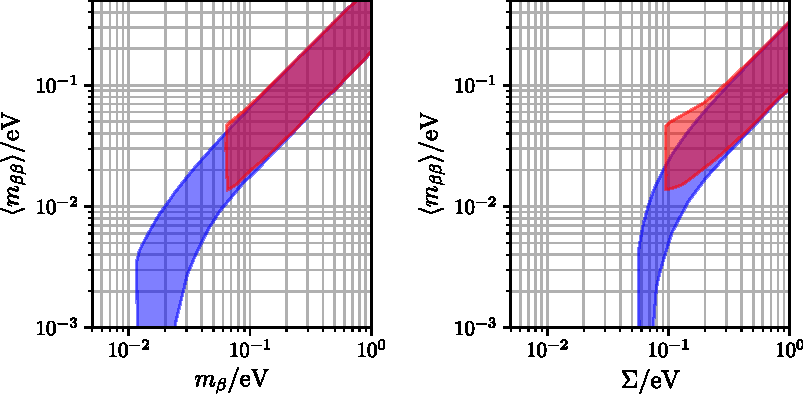
\includegraphics[width=0.8\linewidth]{plots/theory/nu-mass-observables.pdf}
  \caption{%
    The effective mass \mbb\ versus the kinematic neutrino mass observable
    \mb, and the cosmological observable $\Sigma$. The neutrino
    oscillation parameters are varied within their $3\sigma$ ranges. The blue
    (red) area is for the normal (inverted) mass ordering. Taken
    from~\cite{Dolinski2019}.
  }\label{fig:nbb:mass-obs}
\end{figure}

\blocktitle{decay \\ rate}
As we have seen in \cref{eq:nbb:0nudecayrate}, the \onbb\ decay rate can be still
factorized to a good approximation into a phase space factor and a nuclear part, times a
factor encoding the new physics effects generated beyond the Standard Model (the effective
mass in the case of the standard interpretation). Considerations about the theoretical
evaluation of \psft\ and \nmet\ in \cref{sec:nbb:2nbb} are still largely valid for \onbb.
The phase space factor \psfz\ is of the order of $10^{-25}$~yr$^{-1}$ and can be
calculated to a satisfying degree of accuracy~\cite{Kotila2012, Stoica2013} (for \gesix\
it is ${\sim}2.3 \cdot 10^{-15}$~yr$^{-1}$), while nuclear term \nmez\ estimations are in
the 1--10 range but remain terribly affected by large error bars. The situation for the
latter is depicted in \cref{fig:nbb:nme}. As already mentioned in \cref{sec:nbb:2nbb}, the
quenching problem affects also \onbb. Recent studies suggest that there might be less
quenching needed (not more than 20--30\%) in processes with large momentum transfer such
as \onbb~\cite{?}, but there is not yet consensus in the literature. A reduced $g_A$
implies a longer \thalfzero, which is undesirable for experimental searches.  Since no
neutrinos are emitted during the process, the experimental signature of \onbb\ is a
Dirac-delta function at \qbb\ in the summed energy spectrum of the decay products
(\cref{fig:nbb:spectra}).

\begin{figure}
  \centering
  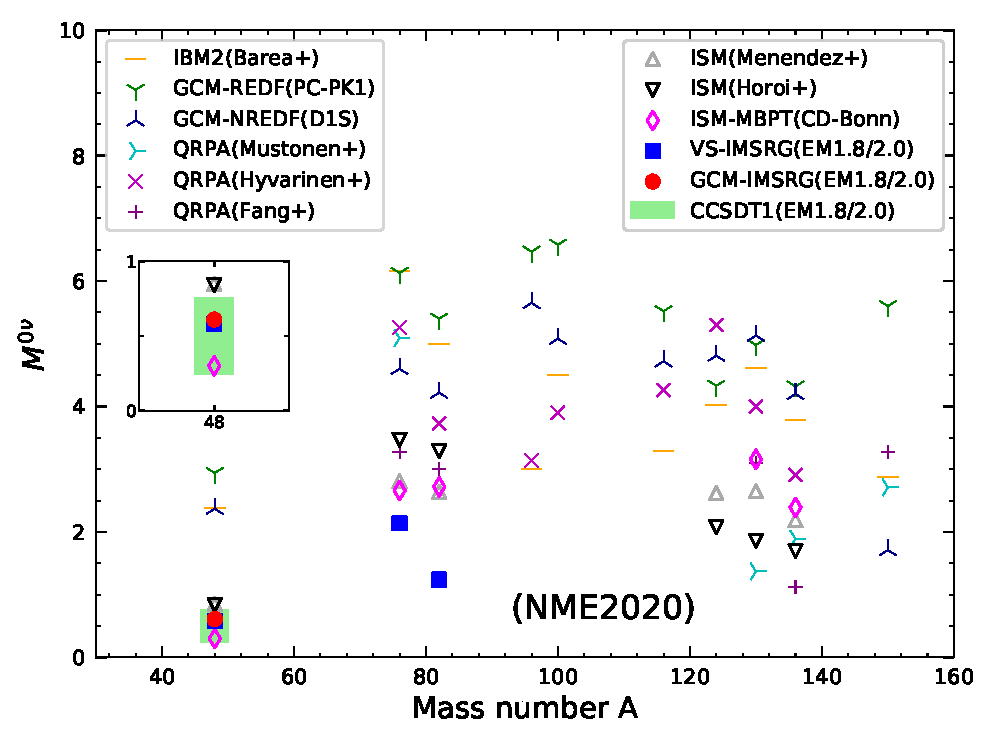
\includegraphics[width=0.6\textwidth]{plots/theory/0nbb-nme.pdf}
  \caption{%
    A representative compilation of nuclear matrix element calculations with an unquenched
    $g_A=1.27$ for different isotopes. Taken from~\cite{Yao2020}.
  }\label{fig:nbb:nme}
\end{figure}

\blocktitle{experimental \\ limits}
A compilation of the current most stringent experimental bounds on \thalfzero\ and \mbb\
from \gesix, \nuc{Te}{130} and \nuc{Xe}{136} is given in \cref{tab:nbb:0nbb-lim}. The
\gerda, \kamlandzen\ and CUORE experiments are competing in setting the best half-life
lower limits and \mbb\ upper limits. The experimental program to search for \onbb\ decay
is presented more in detail in \cref{sec:nbb:exp}.

\begin{table}
  \centering
  \caption{%
    Compilation of current most stringent 90\% C.L.~experimental bounds on
    \thalfzero\ and \mbb\ from \gesix, $^{130}$Te and $^{136}$Xe experiments. A
    value of $g_A \simeq 1.27$ is used.
  }\label{tab:nbb:0nbb-lim}
  \begin{tabular}{lcccc}
  \toprule
  Experiment                               & Isotope               & Exposure (\kgyr) & \thalfzero\ (\powtenyr{25}) & \mbb\ (meV)  \\
  \midrule
  \gerda~\cite{Kermaidic2020,Agostini2021} & \mr{2}{\gesix}        & 127.2            & 18                          & 80--102      \\
  \majorana~\cite{Alvis2019}               &                       & 26               & 2.7                         & 200--430     \\
  \midrule
  \cuoricino~\cite{Andreotti2010}          & \mr{3}{\nuc{Te}{130}} & 19.8             & 0.28                        & 300--710     \\
  CUORE-0~\cite{Alfonso2015}               &                       & 9.8              & 0.24                        & 270--760     \\
  CUORE~\cite{Adams2019}                   &                       & 372.5            & 3.2                         & 75--350      \\
  \midrule
  EXO-200~\cite{Anton2019}                 & \mr{2}{\nuc{Xe}{136}} & 234.1            & 3.5                         & 93--286      \\
  \kamlandzen~\cite{Gando2016}             &                       & 594              & 10.7                        & 61--165      \\
  \bottomrule
\end{tabular}

\end{table}

\section{Neutrinoless double-beta decay with Majoron emission}%
\label{sec:nbb:0nbbx}

As mentioned in \cref{sec:nbb:0nbb}, the Majorana nature of the neutrino leads
to the violation of the baryon-lepton number $U{(1)}_{B-L}$ by two units.
Assuming that the symmetry is global and its breaking occurs spontaneously, a
massless Nambu-Goldstone boson, called the Majoron (denoted~$\upchi$), must exist
in the theory~\cite{Chikashige1981, Schechter1982b, Gelmini1981, Georgi1981,
Mohpatra2004}.  Models with massless Majorons have been studied extensively in
the `80 where the Majoron is either a singlet~\cite{Chikashige1981} or part of
a doublet or a triplet~\cite{Gelmini1981, Georgi1981}. However, the last two
possibilities can be ruled out by measurements of the $Z_0$ invisible width at
particle colliders, because of the coupling of the $Z_0$ to the
Majoron~\cite{Berezhiani1992}. All the mentioned models predict neutrinoless
double-beta decay with Majoron emission:
\[
  0\upnu\upbeta\upbeta\upchi:\quad
    \mathcal{N}(A,Z) \longrightarrow \mathcal{N}(A,Z+2) + 2e^- + \upchi
\]
the Feynman diagram is shown in \cref{fig:nbb:majfeydiag}, left. Since the
coupling strength of the singlet `seesaw' Majoron is proportional to $m_{\upnu} /
\Lambda$, where $\Lambda$ is the lepton number breaking energy scale (i.e.~the
heavy right-handed neutrino mass in the seesaw mechanism), obtaining observable
decay rates for \onbbx\ and preserving existing bounds on neutrino masses would
require a severe fine-tuning in the theory~\cite{Burgess1993, Burgess1994}.
\newpar
Another possibility for neutrinoless double-beta decay with Majoron emission
arises in supersymmetric models with R-parity violation~\cite{Masiero1990,
Mohpatra2004}, in which the emission of two Majorons is also
allowed~\cite{Mohpatra1988}:
\[
  0\upnu\upbeta\upbeta\upchi\upchi:\quad
    \mathcal{N}(A,Z) \longrightarrow \mathcal{N}(A,Z+2) + 2e^- + 2\upchi
\]
See \cref{fig:nbb:majfeydiag} (right) for the Feynman diagram of the process.
\newpar
To overcome the fine-tuning problem, many alternative models have been
developed starting from the `90. In this class of models, the term `Majoron'
refers more generically to a light or massless boson, not necessarily a
Goldstone scalar boson, that couples to the neutrino. There are models which
foresee Majorons carrying leptonic charge, thus assuring lepton number
conservation and forbidding \onbb. For the case of Majorons with $L = −2$,
\onbbx\ is expected~\cite{Burgess1993}, while $L = −1$ for the Majoron leads to
\onbbxx~\cite{Burgess1994}. Other models make use of a vector Majoron which
becomes the longitudinal component of a massive gauge boson emitted in
double-beta decay~\cite{Carone1993}, which we will also refer to as `Majoron'
in the latter. A decay process that involves the emission of two Majorons is
also possible~\cite{Bamert1995}.  In~\cite{Mohpatra2000}, the model of a `bulk'
Majoron has been proposed within models featuring extra dimensionalities
(`brane-bulk' scenario for elementary-particle physics).
\newpar
For the sake of completeness, it has to be mentioned that in recent years
models with massive Majorons (\cite{Blum2018} and references therein) have
progressively gained popularity, being this kind of Majoron an appealing dark
matter particle candidate. This hypothesis remains however largely untested
from the experimental point of view, because of the additional level of
complexity added to the double-beta event analysis.

\begin{figure}
  \centering%
  \makebox[\textwidth]{%
    \includegraphics[width=0.5\textwidth]{plots/theory/0nbbxfey.pdf}%
    \includegraphics[width=0.5\textwidth]{plots/theory/0nbbxxfey.pdf}%
  }
  \caption{%
    Feynman graphs for neutrinoless double-beta decay with single (right) and double
    (left) Majoron emission.
  }\label{fig:nbb:majfeydiag}
\end{figure}

\blocktitle{decay \\ rate}
Independently of the model, the decay rate for double-beta decay with Majoron emission can
be factorized as:
\begin{align*}
  \Gamma^{0\upnu\upchi}  &= g_\alpha^2 \cdot G_\alpha^{0\upnu\upchi}(Q_{\upbeta\upbeta}, Z)
    \cdot |M_\alpha^{0\upnu\upchi}|^2 \\
  \Gamma^{0\upnu\upchi\upchi} &= g_\alpha^4 \cdot G_\alpha^{0\upnu\upchi\upchi}(Q_{\upbeta\upbeta}, Z)
    \cdot |M_\alpha^{0\upnu\upchi\upchi}|^2 \;,
\end{align*}
where \ga\ is the effective coupling constant and $\alpha$ denotes the considered
model. The phase space factors can be parametrized as a function of \qbb, the sum kinetic
energy of the two electrons emitted in the decay $K$ and the spectral index $n$:
\[
  G_\alpha^{0\upnu\upchi(\upchi)}(Q_{\upbeta\upbeta}, Z)
    \sim {(Q_{\upbeta\upbeta} - K)}^n \;.
\]
$n = 5$ corresponds to the standard \nnbb\ (i.e.~\cref{eq:nbb:stdmodel}) whereas \onbbx\
can have $n = 1, 2, 3$ and \onbbxx\ can have $n = 3, 7$, depending on the model. As a
consequence, the energy spectrum of the two emitted electrons allows to distinguish the
different models. The energy spectra for all modes of the Majoron emitting double beta
decay are shown in \cref{fig:nbb:majorons-spectra}.

% \begin{table}
%   \centering
%   \caption{%
%     Compilation of up-to-date calculations of phase-space factors
%     \psfmajo~\cite{Kotila2015} and nuclear matrix elements \nmemajo\ for various
%     Majoron-emitting \onbb\ modes and isotopes.
%   }\label{tab:nbb:0nbbx-psf-nme}
%   \begin{tabular}{lcccc}
  \toprule
          & \mc{4}{\psfmajo\ [\powtenyr{-1}] / \nmemajo} \\
  \cmidrule{2-5}
              & $n=1$        & $n=3$        & $n=3$        & $n=7$      \\
  Isotope     & \onbbx\      & \onbbx\      & \onbbxx\     & \onbbxx\   \\
  \midrule
  \gesix\     & \fillme{tbd} & \fillme{tbd} & \fillme{tbd} & \fillme{tbd} \\
  $^{136}$Xe  & \fillme{tbd} & \fillme{tbd} & \fillme{tbd} & \fillme{tbd} \\
  $^{100}$Mo  & \fillme{tbd} & \fillme{tbd} & \fillme{tbd} & \fillme{tbd} \\
  $^{82}$Se   & \fillme{tbd} & \fillme{tbd} & \fillme{tbd} & \fillme{tbd} \\
  $^{116}$Cd  & \fillme{tbd} & \fillme{tbd} & \fillme{tbd} & \fillme{tbd} \\
  $^{48}$Ca   & \fillme{tbd} & \fillme{tbd} & \fillme{tbd} & \fillme{tbd} \\
  $^{150}$Nd  & \fillme{tbd} & \fillme{tbd} & \fillme{tbd} & \fillme{tbd} \\
  $^{130}$Te  & \fillme{tbd} & \fillme{tbd} & \fillme{tbd} & \fillme{tbd} \\
  $^{96}$Zr   & \fillme{tbd} & \fillme{tbd} & \fillme{tbd} & \fillme{tbd} \\
  \bottomrule
\end{tabular}

% \end{table}

\begin{figure}
  \centering
  \includegraphics{plots/theory/majorons-spectra.pdf}
  \caption{%
    Two-electron energy spectra from different models (labeled by the spectral index $n$,
    see text) of double-beta decay of \gesix, including the standard \nnbb, the
    Lorentz-violating mode \nnbblv\ and the Majoron emitting modes.  Analytic formulas,
    obtained with the Primakoff-Rosen approximation, for the Fermi function are taken
    from~\cite{Tretyak1995, Tretyak2002}.
  }\label{fig:nbb:majorons-spectra}
\end{figure}

\blocktitle{experimental \\ limits}
A compilation of the most recent experimental 90\% C.L.~lower limits on the half-life of
Majoron-emitting \onbb-decay for several nuclei is given in \cref{tab:nbb:0nbbx-lim}. To
compare the experimental sensitivity, the upper limit on \ga\ is calculated for the spectral
index $n=1$, for which the half-life limit is usually higher. Phase space factors
\psfmajo\ are taken from~\cite{Kotila2015}, nuclear matrix elements \nmemajo\
from~\cite{Engel2017}. The most stringent limits at the moment are for \nuc{Xe}{136} from
EXO-200 and \kamlandzen.

\begin{table}
  \centering
  \caption{%
    A compilation of the current 90\% C.L.~lower limits on Majoron-emitting \onbb\ modes
    as set by the \gerda, EXO-200, KamLAND-Zen and NEMO-3 experiments for different
    isotopes. The limit on the coupling constant \ga\ for $n=1$ is reported, as calculated
    with phase-space factors from~\cite{Kotila2015} and most up-to-date nuclear matrix
    elements~\cite{Engel2017}. \ga\ limits for the other indices and different models can
    be found in the references.
  }\label{tab:nbb:0nbbx-lim}
  \begin{tabular}{lcccccccc}
  \toprule
                                      &               &                  & \mc{4}{\thalfmajo\ (\powtenyr{21})} &             \\
  \cmidrule{4-7}
  Experiment                          & Isotope       & Exposure (\kgyr) & $n=1$ & $n=2$ & $n=3$ & $n=7$       & $g_\alpha$  \\
  \midrule
  \gerda~\cite{Agostini2015a}         & \gesix\       & 20.3             & 420   & 180   & 80    & 30          & \fillme{tbd}\\
  EXO-200~\cite{Albert2014a}          & \nuc{Xe}{136} & 100              & 1200  & 250   & 27    & 6.1         & \fillme{tbd}\\
  \kamlandzen~\cite{Gando2012}        & \nuc{Xe}{136} & 36.8             & 2600  & 1000  & 250   & 11          & \fillme{tbd}\\
  NEMO-3~\cite{Arnold2013,Arnold2019} & \nuc{Mo}{100} & 34.3             & 44    & 9.9   & 4.4   & 1.2         & \fillme{tbd}\\
  NEMO-3~\cite{Arnold2018}            & \nuc{Se}{82}  & 4.9              & 37    & --    & --    & --          & \fillme{tbd}\\
  NEMO-3~\cite{Arnold2016}            & \nuc{Cd}{116} & 2.16             & 8.5   & --    & --    & --          & \fillme{tbd}\\
  NEMO-3~\cite{Arnold2016a}           & \nuc{Ca}{48}  & 0.037            & 4.6   & --    & --    & --          & \fillme{tbd}\\
  NEMO-3~\cite{Arnold2016b}           & \nuc{Nd}{150} & 0.19             & 30    & --    & --    & --          & \fillme{tbd}\\
  NEMO-3~\cite{Arnold2011}            & \nuc{Te}{130} & 2.31             & 16    & --    & --    & --          & \fillme{tbd}\\
  NEMO-3~\cite{Argyriades2009}        & \nuc{Zr}{96}  & 0.031            & 1.9   & 0.99  & 0.58  & 0.11        & \fillme{tbd}\\
  \bottomrule
\end{tabular}

\end{table}

\section{Lorentz-violating two-neutrino double-beta decay}%
\label{sec:nbb:2nbbLV}

Since the Standard Model of Particle Physics is known to provide a successful description
of most physics at low energies, compared to the Planck scale $m_p {\sim}10^{19}$~GeV, any
signal of new physics must appear at low energies in the form of an effective quantum
field theory containing the Standard Model.  The general effective quantum field theory
constructed from the latter and allowing for arbitrary coordinate-independent Lorentz
violation is called the Standard Model Extension~\cite{Colladay1997, Colladay1998}. As an
effective field theory it provides a link to the Planck scale through operators of
non-renormalizable dimension. The Lagrangian of the Standard Model Extension consists of
the usual Standard Model Lagrangian supplemented by all possible terms that can be
constructed with the existing fields and that introduce violations of Lorentz symmetry.
The additional terms have the form of Lorentz-violating operators coupled to vector
coefficients, and they could arise in a variety of ways.
\newpar
All quantum field operators for Lorentz violation involved in the propagation of neutrinos
have been classified and enumerated~\cite{Kostelecky2012}. Most of these can be studied
using neutrino oscillations, which compare the way different neutrinos propagate and
provide interferometric sensitivity to energy differences between
them~\cite{Kostelecky2003, Diaz2014}. Some effects cannot be detected by neutrino
oscillations because they are produced by `oscillation-free' operators that change all
neutrino energies equally. Most of these can instead be studied by comparing neutrino
propagation to other species, such as time-of-flight experiments that match the group
velocity of neutrinos and photons~\cite{Adam2011}.  However, four oscillation-free
operators leave unaffected the neutrino group velocity and cannot be detected in this way.
Instead, they must be accessed through physical processes that involve neutrino
phase-space properties, such as particle decays. These operators are rare examples of
\textit{countershaded} Lorentz violations~\cite{Kostelecky2009}: Relativity-violating
effects that could be enormous compared to ones suppressed by the ratio $m_W/m_P$ and that
nonetheless could have escaped detection to date. These could provide an interesting path
for building models with viable Lorentz violation obviating the typical requirement of a
heavy suppression factor.
\newpar
The four countershaded neutrino operators are of renormalizable mass dimension $d=3$, are
odd under \cpt, and are controlled by coefficients conventionally denoted with
$(a^{(3)}_\text{of})_{jm}$, where $j$ and $m$ are angular-momentum quantum numbers with $j
= 0,1$. Non-zero values of \aofoo\ could produce small deviations in the shape of the
energy spectra of electrons emitted in \b\ and double-\b\ decays~\cite{Diaz2013a}.
Conservation of energy and momentum is assured by taking these four coefficients to be
constant as usual for couplings beyond the Standard Model, so all physics other than
Lorentz and \cpt\ violation is conventional. Dimensional arguments suggest these
coefficients are likely to dominate at accessible energies and can be measured sensitively
in low-energy processes.
\newpar
The anti-neutrino phase space element $\text{d}^3q$ is modified by the presence
of these new operators:
\[
  \omega^2\text{d}\omega\text{d}\Omega \;\longmapsto\;
    f(\omega)\text{d}\omega\text{d}\Omega\;,
\]
where the anti-neutrino function
\(f(\omega)\simeq\omega^2-\frac{1}{2}m_\nu^2-2\omega\delta\omega\)
encodes the Lorentz-violating modifications
\[
  \delta\omega = -\sum_{jm} e^{im\omega_\oplus T_\oplus}
  \mathcal{N}_{jm}{(a_\text{of}^{(3)})}_{jm}
\]
arising from the modified anti-neutrino dispersion relation~\cite{Kostelecky2012} $\omega
= |\vec{q}| + m_\nu^2 / |\vec{q}| + \delta\omega$. The sidereal time $T_\oplus$
controls the harmonic variation of the anti-neutrino function in the laboratory produced
by the Earth sidereal rotation at frequency $\omega_\oplus \simeq
2\pi/(23\text{h}~56\text{min})$.  The factors $\mathcal{N}_{jm}$ contain information about
the direction of propagation of the anti-neutrinos, expressed relative to the canonical
sun-centered frame of reference~\cite{Bluhm2003, Kostelecky2002}.

\blocktitle{decay \\ rate}
Following the same procedure and adopting the necessary approximations as in the
conventional two-neutrino double-beta decay (\cref{sec:nbb:2nbb}), one can integrate over
all orientation, which implies that only isotropic effects are observable and hence that
the residual spectrum depends only on $\aofM \equiv \aofooM/\sqrt{4\pi}$. After a suitable
change of integration variables and defining the sum of kinetic energies $K=T_1+T_2$ for
the two electrons, the electron sum spectrum reads
\begin{equation}\label{eq:nbb:totwidth}
  \begin{split}
    \frac{\text{d}\Gamma}{\text{d}K} = &
      \Lambda \cdot (K^5 + 10K^4 + 40K^3 + 60K^2 + 30K) \\
      & \times\left[{(Q_{\beta\beta} - K)}^5 + 10 \aofM {(Q_{\upbeta\upbeta} - K)}^4\right] \;. \\
  \end{split}
\end{equation}
The total decay rate can be therefore expressed as an addition of two separate
rates through a perturbation:
\[
  \Gamma = \Gamma_0 + \delta\Gamma = g_A^4 |m_e c^2 \mathcal{M}^{2\upnu}|^2 (G^{2\upnu} +
  \delta G^{2\upnu}) \;,
\]
where the first term is \cref{eq:nbb:stdmodel} and the second one is the perturbation
introduced by Lorentz violation. Detailed calculations can be found
e.g.~in~\cite{Nitescu2020}. The summed-electron energy spectrum generated by the
perturbative term is depicted in \cref{fig:nbb:majorons-spectra}. The proportionality
between the decay rate represented by $\Gamma_0$ (i.e.~the standard \nnbb\ decay
amplitude) and the decay rate relative to the perturbation $\delta\Gamma$ is set by the
\aof\ coefficient:
\[
  \frac{\delta\Gamma}{\Gamma_0} = \frac{\aofM}{\mathcal{R}} \;.
\]
Values for the $\mathcal{R}=\aofM G^{2\upnu} / \delta G^{2\upnu}$ coefficient have been
computed in~\cite{Nitescu2020} using radial solutions of the Dirac equation to express the
Fermi function $F(Z,E)$.

\blocktitle{experimental \\ limits}
Conservative constraints on $|(a_\text{of}^{(3)})_{j0}|$ coefficients have been placed
using published results from the Troitsk and Mainz experiments studying the endpoint of
the tritium beta decay energy spectrum~\cite{Diaz2013}. An outside analysis of data from
the two experiments gives $|(a_\text{of}^{(3)})_{j0}| < 2 \cdot 10^{-8}$~GeV for both
$j=0,1$.  Constraints on the values of \aof\ have also been extracted from studies of
threshold effects in pion and kaon decays~\cite{Kostelecky2012}, yielding $\aofM < 1.9
\cdot 10^{-7}$~GeV as the best upper limit.  Since many double-beta experiments have now
accumulated high-statistic \nnbb\ datasets, constraints on \aof\ has been recently posed
with \nuc{Te}{130}, \nuc{Xe}{136} and \nuc{Mo}{100}. Published limits are summarized in
\cref{tab:nbb:2nbblv-lim}.

\begin{table}
  \centering
  \caption{%
    Compilation of current experimental bounds at 90\% C.L.~on the Lorentz-violating \aof\
    coefficient from double-beta decay.
  }\label{tab:nbb:2nbblv-lim}
  \begin{tabular}{lccc}
  \toprule
  Experiment                  & Isotope    & Exposure (\kgyr) & \aof\ (GeV) \\
  \midrule
  CUPID-0~\cite{Azzolini2019} & $^{130}$Te & 9.95             & $< 4.1 \cdot 10^{-6}$           \\
  EXO-200~\cite{Albert2016}   & $^{136}$Xe & 100              & $\in [-2.65, 76] \cdot 10^{-5}$ \\
  NEMO-3~\cite{Arnold2019}    & $^{100}$Mo & 34.3             & $\in [-4.2, 3.5] \cdot 10^{-7}$ \\
  \bottomrule
\end{tabular}

\end{table}

\section{From theory to the experimental practice}%
\label{sec:nbb:exp}

The primary focus of experiments that involve double-beta decay is the search for the
neutrinoless decay mode, by far the most important compared to other processes. The
observables in direct searches of \onbb\ are the kinematic parameters of the two emitted
electrons. A typical experiment measures the total energy of the two electrons (the only
observable that is both necessary and sufficient for discovery) and may have the
capability to reconstruct the electron tracks in order to reject background events with
different event topologies. Since \qbb\ is usually known to a high degree of accuracy and
the \onbb\ signature is a mono-energetic peak at \qbb, the signal search is performed in a
narrow energy window defined by the energy resolution of the detector.

\blocktitle{background \\ level}
The number of signal counts in this Region Of Interest (ROI) depends linearly on the
detector signal efficiency $\epsilon$, the active mass $M$, the measurement time $t$ and
the isotopic fraction of the double-beta emitter $a$.  These are the quantities that
usually play a fundamental role when designing an experiment. The sensitivity to the
half-life \thalfzero\ scales linearly with the number of candidate signal counts in the
ROI, but the dependence is weaker if some of them are background counts. Two experimental
regimes can be defined:
\begin{equation}\label{eq:nbb:bkglevel}
  T^{0\upnu}_{1/2} =
    \begin{cases}
      a M \epsilon t & \text{background-free} \\
      a \epsilon \sqrt{\frac{M t}{B \Delta{E}}} & \text{with background} \;, \\
    \end{cases}
\end{equation}
where $B$ is the `background index', namely the number of background events normalized to
the width of the ROI, source mass and measurement time. This expression clearly shows the
advantage of a background-free experiment, since the \thalfzero\ scales linearly with $t$
as opposed to $\sqrt{t}$ in the presence of backgrounds. The background-free condition is
effectively realized when the expected number of background events in the ROI in the
measurement time $t$ is less than one:
\[
  M \cdot T \cdot B \cdot \Delta{E} < 1 \;.
\]

\blocktitle{isotope \\ choice}
Not all the double-beta emitters that exist in Nature can be effectively employed to
search for \onbb. As it can be clearly understood from \cref{eq:nbb:bkglevel}, an ideal
isotope should have a high isotopic abundance $a$, should be available in large quantities
$M$ as high-resolution $\Delta{E}$ detectors under low background conditions $B$. Other
relevant isotope features are a low \nnbb\ decay rate to mitigate the occurrence of
background events in the ROI, and a high \qbb\ to avoid backgrounds from primordial
radioisotopes which are naturally present in construction materials. Moreover, the
detection efficiency $\epsilon$ can be drastically enhanced if the source material is
integrated in the detector medium.  A good double-beta emitter should also be readily
available in its natural form and have a high natural abundance, to reduce the cost of the
experiment. If natural abundance is high enough, isotope enrichment might also be
unnecessary, as demonstrated in the case of $^{130}$Te~\cite{Alduino2017}.

\blocktitle{backgrounds}
To achieve the ambitious goal of operating in a background-free regime, the
next-generation experiments need to fight against many different background sources. Here
a short summary of the main experimental issues concerning this topic is given. The only
irreducible background to \onbb\ signal searches is given by \nnbb\ events. A careful
isotope and detector technology choice can mitigate the impact of such a contribution,
since the number of \nnbb\ events that can leak in the ROI reduces with increasing energy
resolution.  Solar neutrino interactions are also expected to be relevant in tonne-scale
detectors, and the respective background contribution can be mitigated by a high mass
loading of the decaying isotope in the target medium. As already mentioned, radioisotopes
from the uranium and thorium decay chains are ubiquitous in construction materials and
their presence must be kept to a minimum. Material radio-purity must be kept high during
production and later on before installation, to avoid, among the others, contamination by
exposure to \Rn. Natural radioactivity from components far away from the active source,
e.g.~rock walls of an underground laboratory, can be passively screened with clean lead or
copper, water or cryogenic liquid. The latter two options allow the shielding medium to
serve also as an active shield vetoing background events. Cosmic rays can also induce
several type of backgrounds. Prompt muon interactions typically deposit large amount of
energy in detectors and can be easily vetoed. Backgrounds coming from secondary neutrons
and cosmogenically-activated isotopes are the main worries. The latter can be avoided by
minimizing the exposure of the active material to cosmic rays on the Earth's surface and
rapidly deploying them underground.

\blocktitle{experimental \\ approaches}
Neutrinoless double-beta decay has a characteristic event topology with the emission of
two $\sim$MeV electrons. Low-density-gas tracking detectors can in principle resolve the
two electron tracks, leaving only the irreducible background from \nnbb\ decay. For
detectors with higher density, such as discrete detectors or liquid scintillator
detectors, these electrons deposit their energy within a few millimeters, allowing a less
powerful but still useful discrimination between `compact' signal-like events and \g\
rays, which are likely to scatter and deposit energy at multiple sites. The difference may
be resolved through discriminating between the `single-site' and `multi-site' events by
pulse-shape discrimination or reconstructed event topology, depending on the position
resolution, as well as the size and type of a given detector.  Some detectors are capable
of particle discrimination through multiple detection channels, e.g.~scintillation and
ionization. This could allow for the identification of \a\ backgrounds. Other
discrimination techniques exploit the spatial distribution of background events, if
consistently different from that of the signal events. If background events coming from
mechanical support materials are concentrated close around them they might be rejected by
an optimized fiducial volume cut, if a monolithic detector is used. In presence of a
discrete detector, instead, multi-detector event cuts can be used to isolate double-beta
point-like events.

\begin{description}[wide]

  \item[Semiconductors] One of the most promising approaches for scaling to tonne-scale
    experiments is using \gesix-enriched High-Purity Germanium (HPGe) detectors, which
    serve as active source and target for \onbb\ at the same time. The main advantages of
    using HPGe detectors are the maturity of the industrial production technologies, their
    intrinsic purity and the superior energy resolution (per-mill level at \qbb).  A clear
    disadvantage of these detectors is their production cost and the low \qbb\ of
    $\sim$2~MeV. The current generation of \gesix\ experiments is constituted by
    \gerda~\cite{Budjas2013} and \majoranademo~\cite{Abgrall2014}, whose collaborations
    are currently joining their efforts into the next-generation LEGEND experimental
    program~\cite{Abgrall2017}. Its first phase, LEGEND-200, is expected to start data
    taking in 2021 while its planned tonne-scale phase LEGEND-1000, aims at $\thalfzeroM
    {\sim}10^{28}$~yr sensitivity.

  \item[Bolometers] Bolometers are cryogenic calorimeters that operate at temperatures of
    $\sim$10~mK. An absorber is connected to the thermal bath via a weak thermal link, and
    the temperature is read out by a sensitive thermometer. Crystal absorbers can be grown
    from many materials that include double-beta decay isotopes, e.g.~TeO$_2$,
    $^{116}$CdWO$_4$, Zn$^{82}$Se, $^{40}$Ca$^{100}$MoO$_4$, Zn$^{100}$MoO$_4$ and
    Li$_2^{100}$MoO$_4$.  Advantages of this detector technology are the intrinsically low
    crystal radioactivity and the high energy resolution. The challenge is to operate a
    large-scale detector at these ultra-low temperatures. Existing projects that exploit
    the bolometric technique are CUORE~\cite{Arnaboldi2002, Artusa2014}, that takes
    advantage of the large natural abundance of \nuc{Te}{130}, CUPID~\cite{Wang2015}, which
    explores the possibility to improve the background rejection in CUORE through active
    particle discrimination, and \textsc{AMoRE}, a \nuc{Mo}{100}-based
    experiment~\cite{Kim2015}. The ultimate sensitivity goal of the CUPID and
    \textsc{AMoRE} tonne-scale program is $\thalfzeroM > 10^{27}$~yr and $\thalfzeroM
    \sim 5 \cdot 10^{26}$~yr, respectively.

  \item[Time Projection Chambers] The time projection chamber (TPC) is an attractive
    detector technology for \onbb-decay searches because of a combination of mass
    scalability and access to multiple background discrimination variables. A TPC takes
    advantage of a detection medium that produces two energy channels: ionization and
    scintillation. The combination of these two signals allows the reconstruction of event
    topology, position, energy and particle type. \nuc{Xe}{136} is a convenient source and
    detector medium for both liquid- and gas-phase TPCs. By operating high-pressure
    gas-phase xenon TPCs in electroluminescent mode, an energy resolution of better than
    0.5\% FWHM at \qbb\ can be achieved. Liquid-phase xenon TPCs, instead, offer maximum
    source density. Since \onbb\ searches focus on low background and good energy
    resolution, single-phase detectors are usually chosen for liquid-phase TPCs. The
    achievable energy resolution is somewhat worse than that of the gas-phase detectors,
    but multi-site background and spatial distribution discrimination work well with
    position resolution achievable at the few-mm level. Notable projects focusing on the
    liquid-xenon single-phase TPC technology to search for \onbb\ are
    EXO-200~\cite{Auger2012} and its proposed tonne-scale successor,
    \textsc{nEXO}~\cite{Kharusi2018}, which aims at $\thalfzeroM {\sim}10^{28}$~yr
    sensitivity.  Planned high-pressure xenon gas-phase TPC projects are
    NEXT~\cite{Lopez-March2017} (\thalfzero\ sensitivity goal $2.8 \cdot 10^{25}$~yr with
    NEXT-100) and \textsc{PandaX-III}~\cite{Chen2016} (\powtenyr{27} sensitivity goal
    within its tonne-scale program). Two-phase liquid-xenon detectors, popular for dark
    matter searches, such as LUX-ZEPLIN~\cite{Akerib2015},
    \textsc{XENON-nT}~\cite{Aprile2017} and the future DARWIN~\cite{Aalbers2016} might
    also have the capability to search for \onbb\ decay.

  \item[Scintillators] The main appeal of organic scintillators for \onbb\ searches is
    their mass scalability, despite their poor energy resolution.  Another advantage of
    liquid target masses is the possibility to remove contaminants online. A notable
    experiment exploiting this detection approach is \kamlandzen, which loaded nearly
    400~kg of enriched xenon (\kamlandzen\ 400, Phase~II). The collaboration is currently
    starting the new KamLAND-Zen 800 phase, that will load 750~kg of enriched xenon. In
    the longer term, the KamLAND-Zen collaboration plans to deploy over a tonne of
    enriched xenon and to reduce the \nnbb-decay background in the signal region of
    interest by improving the detector resolution in the \textsc{KamLAND2-Zen} experiment and
    reaching a \thalfzero\ sensitivity of ${\sim}2 \cdot 10^{27}$~yr. Searching \onbb\
    decay with $^{130}$Te is the main goal of another liquid scintillator experiment,
    SNO+~\cite{Andringa2015}, which is currently loading its target medium with the source
    isotope~\cite{Paton2019}. Also inorganic CaF$_2$ scintillators have been always
    receiving interest, because of the high $^{48}$Ca \qbb\ of 4.27~MeV. However, finding
    a cost effective process to enrich the isotope, whose natural abundance is only
    $\sim$0.2\%, is still a challenge. The CANDLES series~\cite{Umehara2015} of \onbb\
    searches at the Kamioka Observatory is actively exploring this experimental approach.

  \item[Tracking Calorimeters] The \textsc{SuperNEMO}~\cite{Arnold2010} unique
    experimental program, based on the technology demonstrated by
    NEMO-3~\cite{Arnold2004}, uses a thin foil of source material in the center of a
    sandwich configuration, surrounded first by a low-pressure gas tracking layer to track
    the two \b\ particles and then a calorimetric layer to measure the energy. This type
    of detectors provides superior topological information and is the only detector
    technology capable of measuring the opening angle between the two {\b}s --- one
    observable that can distinguish certain underlying mechanisms for \onbb\ decay. In
    addition, many different isotopes can be formed into foils and studied in the same
    detector configuration. The advantage of this detection approach is the excellent
    background discrimination, which allows to easily reach a zero-background condition.
    However, the low energy resolution does not permit to efficiently discriminate between
    \nnbb\ and \onbb\ events around \qbb, plus the detection efficiency is low (around
    30\%) and the thin source foils are difficult to scale up to large exposures. The
    sensitivity with $^{82}$Se for a full \textsc{SuperNEMO} is projected to be $1.2 \cdot
    10^{26}$~yr.

\end{description}

\chapsummary
\begin{itemize}
  \item Double-beta decay is a rare nuclear decay process in which two electrons and two
    electron anti-neutrinos are emitted. The decay rate can be factorized in a phase space
    factor, that can be calculated to a high degree of accuracy, and a nuclear matrix
    element, which is notoriously much more difficult to evaluate. Several numerical
    approaches to the problem have been proposed, which give inconsistent results. The
    energy spectrum of the two emitted electrons is a continuous distribution between zero
    and the Q-value of the reaction.
  \item Neutrinoless double-beta decay is an hypothetical decay mode in which no neutrinos
    are present in the final state. The occurrence of such a process is connected to the
    fundamental properties of the neutrino and the origin of the our matter-dominated
    universe. The observation of neutrinoless double-beta decay would establish the
    Majorana nature of the neutrino and imply the existence of physics beyond the Standard
    Model. The observable connected to the neutrino mass tested by neutrinoless
    double-beta decay is the so-called `effective Majorana mass'. The experimental
    signature of the decay is a mono-energetic peak in the summed energy spectrum at the
    Q-value. No experiments have reported unambiguous evidence of the existence of the
    decay so far.
  \item Since neutrinoless double-beta decay requires a symmetry breaking in the model, a
    massless bosonic particle, the so-called Majoron, must exist in the theory. Many
    theories predict the presence of Majorons in the final state of the decay process.
    Another hypothetical process is the Lorentz and CPT violating two-neutrino double-beta
    decay, which has been proposed in the framework of the Standard Model Extension. The
    experimental signature of these exotic decay modes is a distortion of the standard
    two-neutrino double-beta decay spectrum, regulated by the coupling constant \ga\ in
    presence of Majorons or the \aof\ coefficient in the case of Lorentz symmetry
    violation.
  \item Several experimental aspects are of fundamental importance when searching for
    neutrinoless double-beta decay in laboratories. The so-called background-free
    condition, in which the sensitivity to the signal scales linearly with exposure time,
    is realized when the expected number of background events at the double-beta decay
    Q-value is less than one. The current and planned experimental program is rich
    and vast. Science collaborations that deploy semiconductors, bolometers, time projection
    chambers, scintillators and tracking calorimeters are challenging each other in
    setting the most stringent limit on the neutrinoless double-beta decay half life, if
    not finding a signal.
\end{itemize}

% vim: tw=90
